\documentclass{article}

\usepackage{graphicx}
\graphicspath{ {images/} }
\usepackage{hyperref}
\usepackage[margin=1in]{geometry}

\title{Student Proposal: Diversity and Inclusion in the Computer Science Department}
\author{
Katie Bramlett$^1$\and
Oliver Broadrick\and
Linnea Dierksheide\and
Alyssa Ilaria\and
Sam Kusner$^2$\and
Catherine Meadows\and
Sreya Nalla$^3$\and
Marshall Thompson\and
Steven Yoon$^4$
}
\date{%
    $^1$Co-Chair, Women in Computer Science\\
    $^2$Vice President, GW Chapter, Association for Computing Machinery\\
    $^3$Senior Class Representative, Women in Computer Science\\
    $^4$President, GW Chapter, Association for Computing Machinery\\
    gw.cs.inclusivity@gmail.com\\
    28 February 2021
}

%\date{\today}

\begin{document}
\maketitle

%\begin{abstract}
%This is the paper's abstract \ldots
%\end{abstract}

\section{Introduction}
To foster a diverse and inclusive community, the Computer Science Department (CSD), 
needs to develop and enforce a plan that is reflective of student beliefs and values.
Written by students, this proposal
provides specific recommendations, goals, and initiatives
to the CSD to constructively improve
inclusivity for all.
When addressing such matters, we recognize and support the importance of 
placing value on voices by including the thoughts and ideas of all students, from all backgrounds.
Therefore, we distributed a survey to gather thoughts and suggestions from students, as well as 
quantitative information. So far, we have
received responses from $63$ students, approximately $25\%$ of CSD undergraduates.

\paragraph{Outline}
The remainder of this document is organized as follows.
Section~\ref{survey} describes the survey and its quantitative results.
Proposed actions are presented in Section~\ref{proposed actions}.

\section{Survey}\label{survey}
To create an accepting, inclusive working and learning environment, we must 
first foster a space for meaningful participation from people of all backgrounds.
Conducting an (optionally) anonymous survey allowed us to articulate a proposal, 
founded upon diverse ideas and perspectives, that outlines a diversity-oriented
strategy for promoting an inclusive culture within the CSD.

The survey was distributed using multiple platforms. Flyers with QR Codes were posted
throughout the fourth floor of the Science and Engineering Hall.
Posts were made in online forums of at least one course
for each undergraduate class (freshman, sophomore, junior, and senior).
Several Undergraduate Teaching Assistants made announcements to their 
students about the survey, projecting the QR Code and giving time
for students to fill it out. Lastly, the Association for Computing Machinery (ACM) and Women 
in Computer Science (WiCS) chapters distributed the survey to their members via email. 


\subsection{Questions}
The survey contained the following $10$ questions:
\begin{enumerate}
\item Please rate the inclusivity of this department based on your experience.	
\begin{itemize}
\item
\emph{The options for this question are the integers $1,2,3,4,5$ 
where $1$ is labeled as "Poor" and $5$ is labeled as "Excellent".}
\end{itemize}
\item Please share any ideas for how we can make our department more inclusive.	
\item If you can identify a problem with the inclusivity of our department but have no ideas for ways to improve it, you are still welcome to share your thoughts here if you would like.	
\item Your name? (only if you want your responses to be publicly associated with your name)	
\item Pronouns?	
\item Gender identity?	
\item Race/ethnic group or groups?	
\item Disability status?	
\item Anything else?	
\item Class? (2022, 2023, 2024, 2025, other?)
\end{enumerate}

\subsection{Quantitative Results}
The survey yielded some interesting quantitative results that can be 
used to further our understanding of these issues.
As of writing, $63$ responses have been submitted in the $6$ days for which the form
has been available.
This is roughly $25\%$ of the $261$ total undergraduates in CSD.
Figure~\ref{gender} shows that females and non-binary students tend to rate inclusivity lower than males.
Figure~\ref{race} shows the average inclusivity rating of several racial 
and ethnic groups.
Finally, Figure~\ref{class} shows a sharp decline in average inclusivity rating with 
expected year of graduation, in other words, with undergraduate class.

\begin{figure}[!h]
\label{gender}
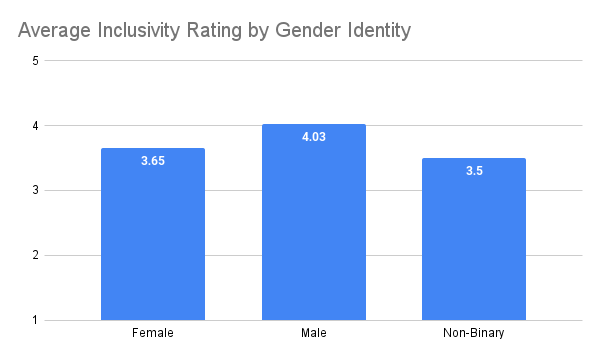
\includegraphics[width=.7\textwidth]{gender_identity.png}
\caption{Mean inclusivity rating by gender identity.
The number of responses that identified themselves in 
one of these categories is respectively 23, 29, and 2.}
\end{figure}
\begin{figure}[!h]
\label{race}
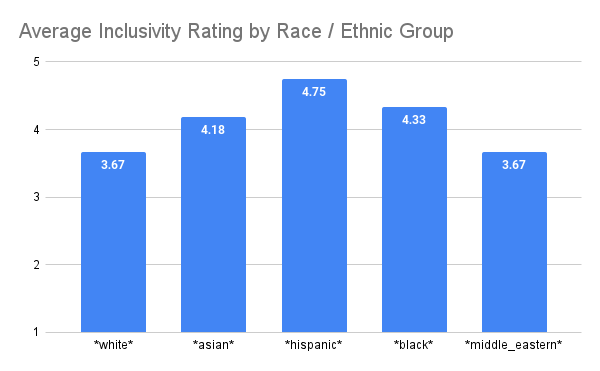
\includegraphics[width=.7\textwidth]{race_ethnic_group.png}
\caption{Mean inclusivity rating by self-described race/ethnic group.
The number of responses that identified themselves in 
one of these categories is respectively 24, 17, 4, 3, and 3.}
\end{figure}
\begin{figure}[!h]
\label{class}
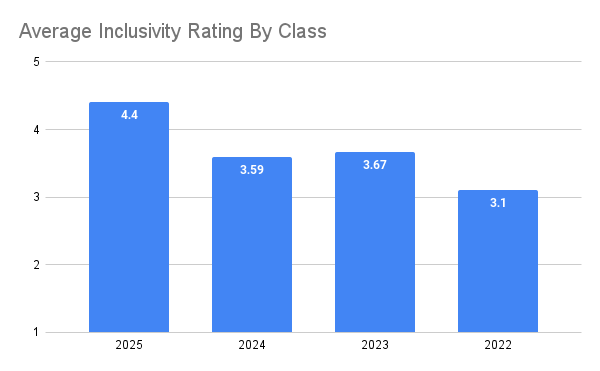
\includegraphics[width=.7\textwidth]{class.png}
\caption{Mean inclusivity rating by undergraduate expected graduation year (by undergraduate class).
The number of responses that identified themselves in 
one of these categories is respectively 20, 22, 6, and 10.}
\end{figure}

\subsection{Qualitative Themes}
Comments from surveyed students covered a range of both positive and negative feedback and ideas. 
Items mentioned by students included
a broad interest in more community engagement events, a desire for increased communication about 
ongoing diversity and inclusion efforts, and active changes to progress towards a more 
diverse student body and faculty. Common themes of dissatisfaction that
were raised included a lack of support for DSS students, unequal treatment 
of CSD organizations, and a belief that certain faculty members lack care and respect
for inclusivity efforts. To address these raised concerns, and using the ideas generated by survey responses,
we propose tangible measures for the CSD to cultivate an inclusive culture in Section~\ref{proposed actions}.

\section{Proposed Actions}\label{proposed actions}
The following items are presented in no particular order.

\subsection{Classroom Environment} 
Active inclusivity efforts in the classroom are necessary to both correct existing disparities as well as to 
establish a tone that prioritizes diversity and inclusion. The efforts listed below should be made explicit by 
professors at the beginning of each course for increased transparency and understanding. 
This includes but is not limited to: 
\begin{itemize}
\item
\emph{Syllabus Diversity \& Inclusion Statement.} 
As with the common religious accommodation, academic integrity, and DSS statements in course syllabi, 
faculty should be required to include a diversity and inclusion statement. 
This statement should provide information about resources available to students related to diversity and inclusion.
A sample statement is as follows: 
\begin{center}
"It is my intent that students from all diverse backgrounds and perspectives be well-served by this course, 
that students' learning needs be addressed both in and out of class, and that the diversity that the students 
bring to this class be viewed as a resource, strength and benefit. It is my intent to present materials and 
activities that are respectful of: gender identity, sexuality, disability, age, socioeconomic status, ethnicity, 
race, nationality, religion, and culture. Your suggestions are encouraged and appreciated. Please let me know ways to 
improve the effectiveness of the course for you personally, or for other students or student groups."
\footnote[1]{
Brown University Diversity and Inclusion Sample Statement Sourced from Clemson University Document "Diversity and Inclusion Syllabus Statements"
published at "clemson.edu".

}
\end{center}
\item
\emph{Assigning Groups for Class Projects.} 
Professors should not be allowed to assign groups based on academic ability, gender, sexuality, race, disability
status, or religion.
Groups should be assigned accordingly: (a) randomly, (b) by the choices of students, or (c) in accomodation of special 
cases including but not limited to as a protective measure in the event of prior discriminatory behavior within a group.
\item
\emph{Group Work Evaluations.} Peer evaluations for group assignments should be given after all group assignments 
or, in the case of long-term projects, given periodically throughout the term. These evaluations should include a 
section that specifically asks about inclusion within the group dynamic (i.e. Are your group members treating 
you with respect? Do you feel like your thoughts and contributions are valued by your group members?). Professors 
should review these evaluations in a timely manner and engage with groups who identified issues. 
\item
\emph{Anonymous Reporting.} 
Students should have an accessible platform for (optionally) anonymous feedback for each course. 
This could manifest as an anonymous form for reporting biased behaviors, giving feedback about inclusion efforts 
in the classroom, etc. This feedback should be frequently monitored by the instruction team and addressed as soon 
as possible. 
\item 
\emph{Office Hours.} 
Office hours, often hosted in casual, common spaces where other students may linger, 
can potentially breed intimidating, exclusive environments. In order to enhance the accessibility of 
instructional team help during office hours, the CSD should assist instruction team members in reserving 
classroom spaces. Hosting office hours in a classroom setting will improve the ability of instructors to more 
fairly distribute their time to all students in attendance. 

\item
\emph{DSS Students.} 
Professors should have (student-optional) recurring “check-in” meetings with DSS students to 
ensure they have proper resources, to check on their progress, etc.
\end{itemize}

\subsection{Instruction Team Training.} 
Undergraduate Teaching Assistants (UTAs), Learning Assistants (LAs), Graduate Assistants (GAs), and 
professors should receive the same diversity and inclusion training (i.e. group training from the GW Office 
for Diversity, Equity, and Community Engagement) prior to interacting with students as a member of the 
instructional team. 

\subsection{Diversity and Inclusion in our Curriculum} 
The CSD ethics course, required for all Computer Science undergraduate students, 
should include a thorough unit and discussion on diversity and inclusion in computing. 
This includes but is not limited to learning how to recognize and address unconscious bias, why diversity in 
engineering is crucial, opportunities and resources within the CSD, and how to have conversations about diversity 
and inclusion efforts.

\subsection{Undergraduate Research Outreach} 
All students should be aware of and feel comfortable in pursuing 
research opportunities with faculty. In order to increase accessibility of faculty and boost awareness, 
opportunities should be displayed and distributed in a public manner. This includes but is not limited to a poster 
displayed outside the CSD office with research opportunities and faculty contact information, publicized research 
talks from students and faculty, announcements to classes about research opportunities.

\subsection{Mindful Pronoun Usage} 
Proper use of gender identity terms, including but not limited to pronouns and prefered names, 
is an essential measure for fostering an inclusive environment. The CSD should normalize pronoun usage in a 
top-down approach, leading by example. This includes but is not limited to including pronouns in faculty biographies 
on the CSD website, in email signatures, in Zoom names, etc. Additionally, when conducting introductions in the 
classroom, faculty can introduce themselves and provide their pronouns and encourage students to do the same, if 
comfortable.

\subsection{Conscious Hiring} 
The Department should make a conscious effort to interview and hire faculty candidates and 
student teaching staff of all backgrounds who share a commitment to upholding diversity and inclusion values. 
This includes asking candidates about their experiences with and interest in implementing inclusivity efforts, as well 
as ensuring our faculty and student instruction teams are reflective of a diverse community.

\subsection{CSD Student Organizations}
\begin{itemize}
\item
\emph{Funding Guidelines.}
The CSD should develop and publicize a clear process for requesting and receiving funding for student organizations.
\item
\emph{Introductions and Equal Treatment.}
To encourage and increase participation in CSD organizations, WiCS, ACM, and future organizations in 
the department should have equal endorsement by faculty. This includes but is not limited to organization introductions by student
representatives at the beginning of freshmen courses, faculty attendance at organization-sponsored events, and equal 
advertisement of organization engagements by the CSD. 
\end{itemize}

\subsection{Diversity \& Inclusion Committee} 
The CSD should form a Diversity and Inclusion Committee, composed of both faculty members and 
student representatives, to monitor progress for the above proposed items and to host regular forums with 
students to source feedback about ongoing initiatives. The faculty advisor(s) for ACM and the faculty advisor(s)
for WiCS will both sit on this committee to increase relations between the CSD and student organizations. 

%\section{Conclusion}\label{conclusion}
\end{document}